\documentclass[xcolor=dvipsnames]{beamer}

\usepackage{pgf}
\usepackage{etex}
\usepackage{tikz,pgfplots}
\usepackage[utf8]{inputenc}
\usepackage[russian]{babel}
\usepackage{xcolor}
\usepackage{graphicx}
\usepackage{MnSymbol}
\usepackage{comment}
\usepackage[utf8]{inputenc}
\usepackage{pdfpages}
\usepackage{listings}
\usepackage{color}
\usepackage{booktabs}
\usepackage{soul}
\usepackage[normalem]{ulem}
\usepackage{tcolorbox}
\usepackage{lipsum}
\usepackage{tikz}
\usepackage{listings}
\usepackage{color}
\usepackage{amsmath,amsfonts}
\usepackage{algorithmic}
\usepackage{algorithm}
\usepackage{array}
%%%%%%%%%%%%%%%%%%%%%%%%%%%%%%%%%%%%%%%%%%%%%%%%%

\usetheme{Antibes}
%\usetheme{Madrid}
%\usecolortheme[named=Maroon]{structure}
\usecolortheme{dolphin}
\usefonttheme{professionalfonts}
\useoutertheme{infolines}
\useinnertheme{circles}

\newtheorem*{bem}{Bemerkung}


\definecolor{dkgreen}{rgb}{0,0.6,0}
\definecolor{gray}{rgb}{0.5,0.5,0.5}
\definecolor{mauve}{rgb}{0.58,0,0.82}

\lstset{frame=tb,
  language=Java,
  aboveskip=2mm,
  belowskip=2mm,
  showstringspaces=false,
  columns=flexible,
  basicstyle={\small\ttfamily},
  numbers=none,
  numberstyle=\tiny\color{gray},
  keywordstyle=\color{blue},
  commentstyle=\color{dkgreen},
  stringstyle=\color{mauve},
  breaklines=true,
  breakatwhitespace=true,
  tabsize=2
}



\newtheorem{remark}{Remark}
% \newtheorem{definition}{Definition}
\newtheorem*{todo}{TODO}
\newtheorem{question}{Вопрос}
\newtheorem*{remark*}{Замечание}
% \newtheorem{theorem}{Theorem}
% \newtheorem{corollary}{Corollary}
\newtheorem*{corollary*}{Corollary}
% \newtheorem{lemma}{Lemma}
\newtheorem*{prop}{Предложение}
\newtheorem{proposition}{Утверждение}

\newcommand{\Id}{\operatorname{Id}}
\newcommand{\HK}[1]{\mathcal{HK}[#1]}
\newcommand{\Real}{\mathbb{R}}
\newcommand{\Exp}{\mathbb{E}}
% \newcommand{\Prob}{\mathbb{P}}
\newcommand{\eps}{\varepsilon}
\newcommand{\boldx}{\boldsymbol{x}}
\newcommand{\Boldx}{\mathbf{x}}
\newcommand{\boldzero}{\boldsymbol{0}}
\newcommand{\boldy}{\boldsymbol{y}}
\newcommand{\Boldy}{\mathbf{y}}
\newcommand{\boldz}{\boldsymbol{z}}
\newcommand{\bolda}{\boldsymbol{a}}
\newcommand{\boldv}{\boldsymbol{v}}
\newcommand{\boldb}{\boldsymbol{b}}
\newcommand{\boldw}{\boldsymbol{w}}
\newcommand{\boldu}{\boldsymbol{u}}
\newcommand{\boldxi}{\boldsymbol{\xi}}
\newcommand{\calP}{\mathcal{P}}
\newcommand{\boldeta}{\boldsymbol{\eta}}
\newcommand{\pinv}[1]{#1 ^ {\mathrm{g}}}
\newcommand{\Ind}[1]{\mathbf{1}_{\left\{#1\right\}}}
\newcommand{\Mat}[2]{\operatorname{Mat}_{#1 \times #2}(\Real)}
\newcommand{\Beps}{B_{\eps}}
\newcommand{\notBeps}{\overline{B}_{\eps}}
%%%%%%%%%%%%%%%%%%%%%%%%%%%%%%%%%%%%%%%%%%%%%%%%%

\title[%
    % Краткое название работы не используется в этой презентации!
    SDE for Generative Modeling 
]{%
    % Полное название работы отображается на титульной странице
    Stochastic Differential Equations for Generative Modeling 
}

\author[%
    % Имя и фамилия автора работы отображаются на каждом слайде в нижнем колонтитуле
    Anton Bolycev 
]{%
    % Имя, отчество и фамилия автора работы отображаются на титульном слайде
    Anton Bolychev 
}

\date[%
    % Дата защиты
    May 2022
]{%
    % Руководитель
    May 2022
}

\institute[%
    % Краткое название организации не используется в этой презентации
    MSU]{%
    % Полное название организации и подразделения
    Moscow State University\\
    Faculty of Mechanics and Mathematics \\
}



\begin{document}
    \begin{frame}
        \titlepage
    \end{frame}
    \section{GAN as Energy-Based Model} 
    \begin{frame}{GAN}
        \begin{align*}
            L_D &= -\mathbb{E}_{x \sim p_{data}} [ \text{log} D(x)] - \mathbb{E}_{z \sim p_z} [\text{log}(1 - D(G(z))] \\    
            L_G &= -\mathbb{E}_{z \sim p_z} [\text{log} D(G(z))]
        \end{align*}
    \end{frame}

    \begin{frame}{GAN as Energy Based Model}
        Assume that Discriminator is suboptimal, i.e. $D = D^*$
        \begin{equation*}
            D(x) = \operatorname*{logit}(d(x)) = \frac{1}{1 + \exp(-d(x))} \approx \frac{p_d(x)}{p_d(x) + p_g(x)}  = \frac{1}{1 + p_g(x)/p_d(x)}
        \end{equation*}
        Thus,
        \begin{equation*}
                p_d^*(x) = p_g(x) e^{d(x)} / K = \exp\left( - (-\log p_g(x) - d(x))\right) / K
        \end{equation*}
        Energy Function. Boltzmann distribution
        \begin{equation*}
            p(z) = \exp(-E(z)) / K 
        \end{equation*}
        Thus, assuming that $x = G(z)$ one can obtain the following equation for Energy for GAN
        \begin{equation*}
            E(z) = -\log p_0(z) - d(G(z))
        \end{equation*}
    \end{frame}

    \begin{frame}{Langevin Dynamics}
        \begin{equation}
            z_{i+1} = z_i - \epsilon/2 \nabla_z E(z) + \sqrt{\epsilon} n, n \sim N(0, I)
        \end{equation}    
         \begin{algorithmic}
            \STATE {\bfseries Input:} N$\in \mathbf{N}_+$, $\epsilon > 0$ 
            \STATE {\bfseries Output:} Latent code $z_N \sim p_t(z)$
            \STATE Sample $z_0 \sim p_0(z)$   
            \FOR{$i=1$ {\bfseries to} $N$}
            \STATE $n_i \sim N(0, 1)$
            \STATE $z_{i + 1} = z_i - \epsilon/2 \nabla_z E(z_i) + \sqrt{\epsilon} n_i$
            \ENDFOR
         \end{algorithmic}
    \end{frame}
    \begin{frame}{Frechet Inception Distance}
        FID can be calculated according to the following formula
        \begin{equation*}
            d_F(\mu, \nu):=\left(\inf _{\gamma \in \Gamma(\mu, \nu)} \int_{\mathbb{R}^n \times \mathbb{R}^n}\|x-y\|^2 \mathrm{~d} \gamma(x, y)\right)^{1 / 2}
        \end{equation*}
    \end{frame}
    \begin{frame}{Results} 
        \begin{center}
            If one apply Langevin Dynamics for pretrained DCGAN on CIFAR10 we observe the following picture
            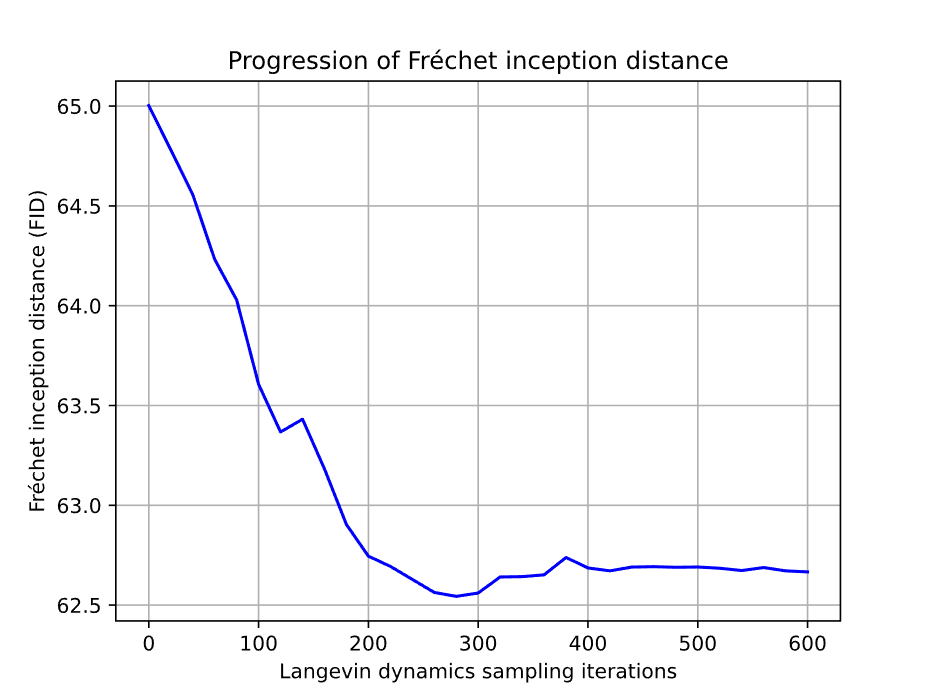
\includegraphics[width=0.7\textwidth]{pics/FID_EBMGAN.png}
        \end{center}
    \end{frame}
    \section{Score-based Generative Modelling through SDE} 
    \begin{frame}{Score-based Generative Modelling through SDE}
        \begin{center}
            The core idea of the paper can be described via the following picture
            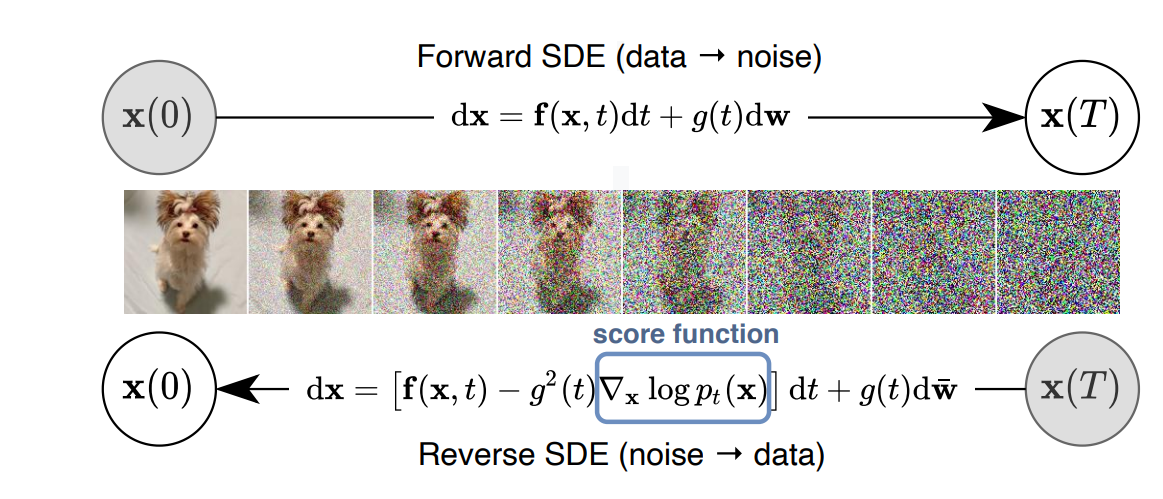
\includegraphics[width=0.7\textwidth]{pics/NoiseDenoise.png}
        \end{center}
    \end{frame}

    \begin{frame}{Score-based Generative Modelling through SDE}
        \begin{center}
            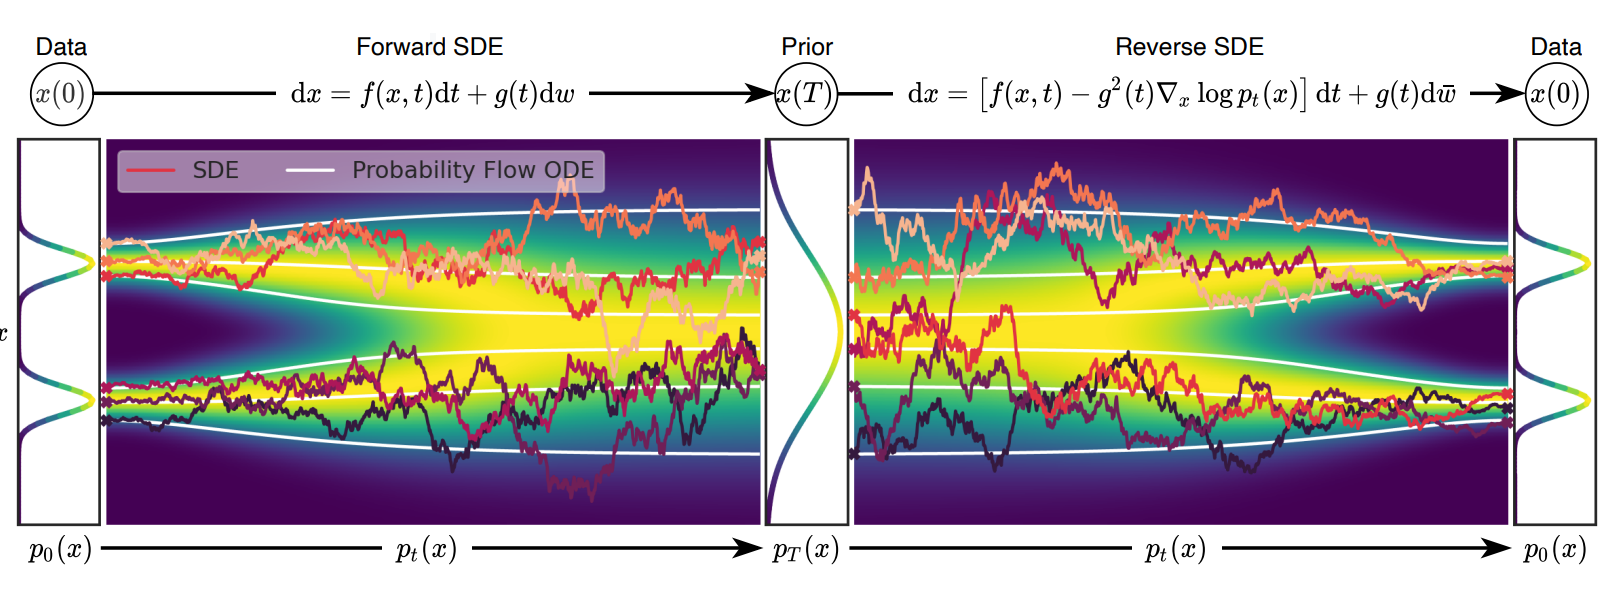
\includegraphics[width=0.7\textwidth]{pics/NoiseDenoise2.png}
        \end{center}
        The main problem is to fit the neural network $\mathbf{s}_{\boldsymbol{\theta}}(\mathbf{x}(t), t)$ such that 
        $$
        \mathbf{s}_{\boldsymbol{\theta}}(\mathbf{x}(t), t) \approx \nabla_{\mathbf{x}} \log p_t(\mathbf{x})
        $$
    \end{frame}

    \begin{frame}{Loss function}
        \begin{multline*}
            \boldsymbol{\theta}^*=\underset{\boldsymbol{\theta}}{\arg \min } \\ \mathbb{E}_t\left\{ 
            \lambda(t) \mathbb{E}_{\mathbf{x}(0)} \mathbb{E}_{\mathbf{x}(t) \mid \mathbf{x}(0)}\left[\left\|\mathbf{s}_{\boldsymbol{\theta}}(\mathbf{x}(t), t)-\nabla_{\mathbf{x}(t)} \log p_{0 t}(\mathbf{x}(t) \mid \mathbf{x}(0))\right\|_2^2\right]\right\} .
        \end{multline*}
        
        where 
        $$
        \lambda \propto 1 / \mathbb{E}\left[\left\|\nabla_{\mathbf{x}(t)} \log p_{0 t}(\mathbf{x}(t) \mid \mathbf{x}(0))\right\|_2^2\right]
        $$
    \end{frame}

    \begin{frame}{2 approaches}
        In $\mathrm{d} \mathbf{x}=\mathbf{f}(\mathbf{x}, t) \mathrm{d} t+g(t) \mathrm{d} \mathbf{w}$ functions $\mathbf{f}$ and $g$ can be arbitrary, so we will consider 2 approaches
        \begin{itemize}
            \item Variance Exploding Approach
            \item Variance Preserving Approach
        \end{itemize}
    \end{frame}

    \begin{frame}{Variance Exploding}
        \begin{itemize}
            \item SDE 
        $$
        \mathrm{d} \mathbf{x}=\sqrt{\frac{\mathrm{d}\left[\sigma^2(t)\right]}{\mathrm{d} t}} \mathrm{~d} \mathbf{w}
        $$
            \item Forward Sampling
            $$
            \mathbf{x}_i=\mathbf{x}_{i-1}+\sqrt{\sigma_i^2-\sigma_{i-1}^2} \mathbf{z}_{i-1}
            $$
        \end{itemize}
    \end{frame}


    \begin{frame}{Variance Preserving}
        \begin{itemize}
        \item SDE 
            $$
        \mathrm{d} \mathbf{x}=-\frac{1}{2} \beta(t) \mathbf{x} \mathrm{d} t+\sqrt{\beta(t)} \mathrm{d} \mathbf{w}
        $$
        \item Forward Sampling
        $$
        \mathbf{x}_i=\sqrt{1-\beta_i} \mathbf{x}_{i-1}+\sqrt{\beta_i} \mathbf{z}_{i-1}
        $$
        \end{itemize}
    \end{frame}

    \begin{frame}{Ancestral Sampling for Variance Preserving}
        $$
        \mathbf{x}_{i-1}=\frac{1}{\sqrt{1-\beta_i}}\left(\mathbf{x}_i+\beta_i \mathbf{s}_{\boldsymbol{\theta}^*}\left(\mathbf{x}_i, i\right)\right)+\sqrt{\beta_i} \mathbf{z}_i, \quad i=N, N-1, \cdots, 1
        $$
    \end{frame}

    \begin{frame}{Reverse Diffusion}
        Given a forward SDE
$$
\mathrm{d} \mathbf{x}=\mathbf{f}(\mathbf{x}, t) \mathrm{d} t+\mathbf{G}(t) \mathrm{d} \mathbf{w}
$$
and suppose the following iteration rule is a discretization of it:
$$
\mathbf{x}_{i+1}=\mathbf{x}_i+\mathbf{f}_i\left(\mathbf{x}_i\right)+\mathbf{G}_i \mathbf{z}_i, \quad i=0,1, \cdots, N-1
$$
Thus, one can propose to discretize the reverse-time SDE
$$
\mathrm{d} \mathbf{x}=\left[\mathbf{f}(\mathbf{x}, t)-\mathbf{G}(t) \mathbf{G}(t)^{\top} \nabla_{\mathbf{x}} \log p_t(\mathbf{x})\right] \mathrm{d} t+\mathbf{G}(t) \mathrm{d} \overline{\mathbf{w}}
$$
which gives the following iteration rule for $i \in\{0,1, \cdots, N-1\}$ :
$$
\mathbf{x}_i=\mathbf{x}_{i+1}-\mathbf{f}_{i+1}\left(\mathbf{x}_{i+1}\right)+\mathbf{G}_{i+1} \mathbf{G}_{i+1}^{\top} \mathbf{s}_{\boldsymbol{\theta}^*}\left(\mathbf{x}_{i+1}, i+1\right)+\mathbf{G}_{i+1} \mathbf{z}_{i+1},
$$
where our trained score-based model $\mathbf{s}_{\boldsymbol{\theta}} *\left(\mathbf{x}_i, i\right)$.
    \end{frame}

    \begin{frame}{Predictor-Corrector Sampling}
        \begin{center}
            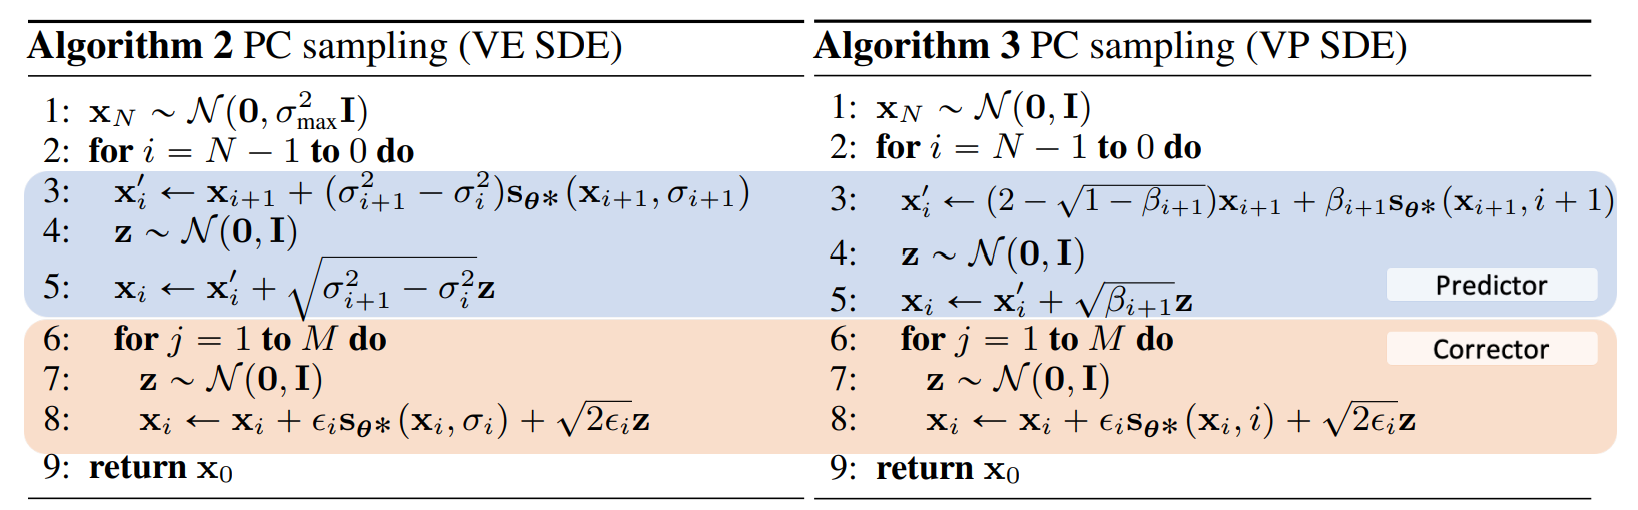
\includegraphics[width=0.7\textwidth]{pics/PC.png}
        \end{center}
    \end{frame}

    \begin{frame}{Results. FID on CIFAR10. VE}            
        \begin{center}
            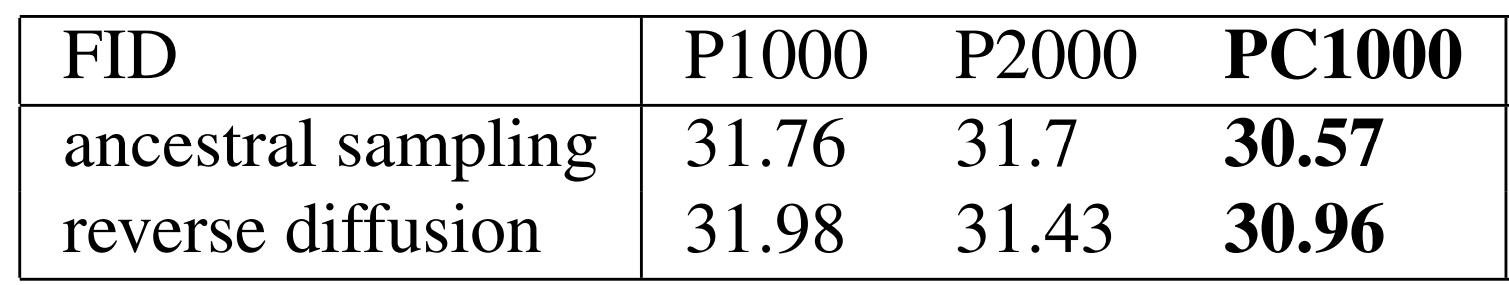
\includegraphics[width=0.7\textwidth]{pics/VE_table.png}
        \end{center}
    \end{frame}


    \begin{frame}{Results. FID on CIFAR10. VP}            
        \begin{center}
            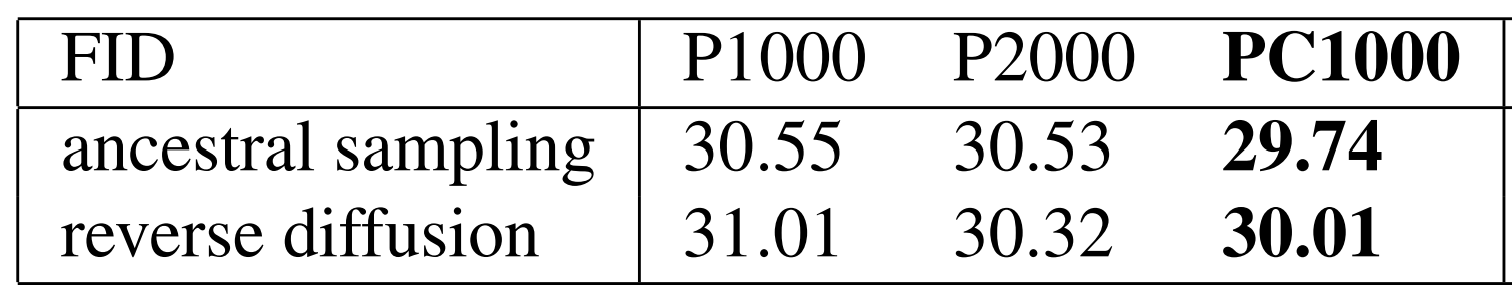
\includegraphics[width=0.7\textwidth]{pics/VP_table.png}
        \end{center}
    \end{frame}

    % \section{Introduction}

In this work we consider noisy modification of the continiuos time HK model with leadership from \cite{leader_hk}.  
    % \section{Model}

In this section we state the noisy modification of the HK model from \cite{leader_hk}. 
The text is almost fully copypasted from the original paper, so it reasonable to make some 
antiplagiat fixes when the need arises.

The system of $N$ interacting agents with one leader with opinions in $\mathbb{R}^d$ is given by
\begin{equation}\label{eq:model_init} 
\left\{\begin{array}{l}
dx_0(t)=u(t)dt \\
dx_i(t)=\left[\sum_{j=1}^N a_{i j}\left(x_j(t)-x_i(t)\right)+c_i\left(x_0(t)-x_i(t)\right)\right] dt + \sigma_i(\mathbf{x}(t) - x_0(t)) dW^i_t,  \text { for } i=1, \ldots, N
\end{array}\right.
\end{equation}
with initial positions $x_j(0)$ such that $\Prob(x_j(0) = x_j^0) = 1$, where $x_j^0 = \operatorname*{const} \in \Real$ for $j=0,1, \ldots, N$. The state of the system, 
representing the agents' and the leader's opinions is 
$\mathbf{x}=\left(x_0, x_1, \ldots, x_N\right) \in \mathbb{R}^{(N+1)}$. We denote the leader by the index 0 and with the index $i=1, \ldots, N$ we denote the $N$ agents. 
The control function, which is a measurable function $t \mapsto u(t) \in \mathbb{R}$ satisfying the constraint $|u| \leq M$, acts only on the leader.
The first term in the dynamics $\sum_{j=1}^N a_{i j}\left(x_j-x_i\right)$, comes from the original HK model. The key idea of the $\mathrm{HK}$ model 
is that each agent updates his opinion by averaging the opinions of the neighbors with a rescaling factor
$$
a_{i j}=a\left(|x_i(t)-x_j(t)|\right)
$$
given by a function $a(r):[0, \infty) \rightarrow[0,1]$ of the distance $r$ between the opinions and representing the interaction rate dependence on the limited confidence domain. 
The function $a=a(r)$ is the following smooth cut-off function
$$
a(r)=a(r ; \delta, \varepsilon) \quad:= \begin{cases}1, & 0 \leq r \leq \delta, \\ \varphi(r), & \delta<r<(\delta+\varepsilon), \\ 0, & (\delta+\varepsilon) \leq r\end{cases}
$$
where $\delta$ is the bounded confidence, $\varphi(r)$ is a decreasing smooth function on $(\delta, \delta+\varepsilon]$, and $\varepsilon>0$ is a parameter of the HK model 
defining the width of the region where the cut-off function decays to zero.
The second term in the dynamics (1) models the action of the leader on the $i$ th agent. A leader can be defined as one agent with a high level of confidence and self-esteem, 
that has the ability to withstand criticism, so that its dynamics is not influenced by the other agents' opinions. The influence of the opinion of the leader on the group opinion 
in decision making is given by the term $c_i\left(x_0(t)-x_i(t)\right)$. The parameter
$$
c_i=\gamma \phi\left(|x_i-x_0|\right)
$$
represents the rate of relationship between the leader and the other agents, 
where $\phi:[0, \infty) \rightarrow(0,1]$ is a smooth non-increasing positive function 
such that $\phi(0)=1$ and $\lim _{r \rightarrow \infty} \phi(r)=\nu > 0$, and where the strength of the opinion 
leader is represented by the parameter $\gamma>0$. In other words the leader has the ability to influence every agent with a factor that is inversely 
proportional to its distance from the agent. The noise part
\[
    \sigma_i(\mathbf{x}(t) - x_0(t)) dW^i_t, 
\]
where $\{W^i_t\}_{i=1}^N$ are independent Weiner processes,  will be considered for different cases
\begin{enumerate}
    \item $\sigma_i(\mathbf{x}(t) - x_0(t)) = \sigma^2$
    \item $\sigma_i(\mathbf{x}(t) - x_0(t)) = \sigma^2(x_i(t) - x_0(t))$
    \item $\sigma_i(\mathbf{x}(t) - x_0(t)) = \sigma^2 h(x_i(t) - x_0(t))$, where $h$ is continuously differentiable function such that 
    \[
        h(0) = 0, \quad |h(\cdot)| \leq 1
    \]
\end{enumerate}
    % \section{Basic concepts and preliminaries} 

Again, copypaste

\textit{
The uncontrolled dynamics of system (1) is governed by local interactions and, in large time, leads to the
formation of clusters. Although, from the mathematical point of view, clusters are a stable configuration for
the system, we focus on the possibility to steer, using the leader’s action on the group, all agents to a same
unique opinion, that is, to have emergence of “consensus”
}

\begin{definition}
We call consensus a configuration in which the states of all agents are equal, i.e,
$$
\mathbf{x}^*=\left(x_0, x_1, \ldots, x_N\right) \in \mathbb{R}^{(N+1)} \quad \text { such that } \quad x_0=x_1=\cdots=x_N .
$$
\end{definition}

Note that it will be convinient for us to reformulate \eqref{eq:model_init} in terms of $y_i(t) := x_i(t) - x_0(t)$ for $i = 1, \ldots, N$:
\begin{equation}\label{eq:model}
    dy_i(t) = \left[-u(t) + \sum_{j=1}^N a_{i j}\left(y_j(t)-y_i(t)\right)-c_i y_i(t)\right] dt + \sigma_i(\Boldy(t)) dW^i_t, \qquad  i = 1, \ldots N,
\end{equation}
where $\Prob(y_j(0) = y_j^0) = 1$ for $j = 1, \ldots, N$ and $\Boldy_0 = (y_1^0, \ldots. y_N^0) \in \Real^N$. 
Thus, the consensus is the configuration $\Boldy^* = (y_1, \ldots, y_n) \in \Real^N$, where $y_1 = \ldots = y_N  = 0$. We will also need
\begin{definition}[modification from \cite{Khasminskii}]
    We will call the solution of the system \eqref{eq:model} exponentially $p$-stable if there exist positive constants $A$ and $\beta$ such that
    \[
       \Exp \|\Boldy(t)\|^p \leq A  \|\Boldy_0\|^p \exp\left\{-\beta t\right\}
    \]
    for all $\Boldy_0 = (y_1^0, \ldots. y_N^0) \in \Real^N$.
\end{definition}
and 
\begin{lemma}[Gronwall-Bellman Lemma \cite{Khasminskii}]\label{lemma:gronwall-bellman}
Let $f(t)$ and $g(t)$ be real-valued functions on $\Real_{\geq0}$ and let $f(t)$ be differentiable on $\Real_{>0}$. If
\[ 
f'(t) \leq f(t) g(t) 
\]
Then for $t \geq 0$
$$
f(t) \leq f(0) \exp \left\{\int_0^t g\left(\tau\right) d \tau\right\} .
$$
\end{lemma}


    % \section{Global stabilization}

\begin{theorem}\label{thm:global-stabilization}
    For all $M \in \Real_{>0}$ there exists smooth control $u(t)$ such that $|u(t)| < M$ for all $t \in \Real_{\geq 0 }$ and 
    \[
        \Exp \|\Boldy(t)\|^2 - \Exp \|\Boldy(s)\|^2 \leq \int_s^t  - \frac{\gamma \nu }{2} \Exp \|\Boldy(\tau)\|^2   + \sum_{i=1}^N \Exp \left[ \frac{\sigma_i(\Boldy(\tau))^2}{2} \right] d\tau 
    \]
\end{theorem}

\begin{proof}
    We consider the control function\footnote{The control function in \cite{leader_hk} has a similar form}
    \[
        u(t) = \alpha(t) \sum_{j=1}^N c_j y_j(t)
    \]
    where $\alpha(t)$ is smooth function of $y_1(t), \ldots, y_N(t)$ such that 
    \[
        \frac{1}{4} \min \left\{\frac{\gamma\phi\left( \max_{i}\left|y_i(t)\right|\right)}{N  \sum_{j=1}^N c_j}, \frac{2 M}{\gamma \sum_i\left|y_i(t)\right|}\right\} \leq \alpha(t) \leq \frac{1}{2} \min \left\{\frac{\gamma\phi\left( \max_{i}\left|y_i(t)\right|\right)}{N  \sum_{j=1}^N c_j}, \frac{2 M}{\gamma \sum_i\left|y_i(t)\right|}\right\} .
    \]
    Note that $u(t)$ is indeed bounded
    \[
        |u(t)| \leq  \alpha(t) \sum_{j=1}^N c_j |y_j(t)| \leq \alpha(t)  \sum_{j=1}^N \gamma |y_j(t)| \leq M
    \]
    Let us apply the Ito's lemma for $\|\Boldy(t)\|^2 = y_1^2(t) + \ldots + y_N^2(t)$:
    \begin{multline*}
        \|\Boldy(t)\|^2 -  \|\Boldy(s)\|^2 = \\ \sum_{i=1}^N\int_s^t \left[ \left(-u(\tau) + \sum_{j=1}^N a_{i j}\left(y_j(\tau)-y_i(\tau)\right)-c_i y_i(\tau)\right) y_i(\tau) + 
        \frac{\sigma_i(\Boldy(t))^2}{2} \right]d\tau + \\ 
        \sum_{i=1}^N  \int_s^{t}\sigma_i(\Boldy(\tau)) y_i(\tau) dW_{\tau}^i
    \end{multline*}
    The expected value of it
    \begin{multline}\label{eq:ExpIto}
        \Exp \|\Boldy(t)\|^2 -  \Exp \|\Boldy(s)\|^2 =  \sum_{i=1}^N \Exp \left[\int_s^t \left(-u(\tau) + \sum_{j=1}^N a_{i j}\left(y_j(\tau)-y_i(\tau)\right)-c_i y_i(\tau)\right) y_i(\tau) d\tau \right] + \\
        \sum_{i=1}^N \Exp \left[ \int_s^{t} \frac{\sigma_i(\Boldy(\tau))^2}{2} d\tau\right] + 0
    \end{multline}
    Let us consider separately
    \[
        \sum_{i=1}^N \Exp \left[\int_s^t \left(-u(\tau) + \sum_{j=1}^N a_{i j}\left(y_j(\tau)-y_i(\tau)\right)-c_i y_i(\tau)\right) y_i(\tau) d\tau \right]
    \]
    We need to rearrange terms in the following way
    \begin{equation}
        \Exp \left[\int_s^t - u(\tau) \sum_{i=1}^N y_i(\tau) + \sum_{i=1}^N \sum_{j=1}^N a_{i j}\left(y_j(\tau)-y_i(\tau)\right)y_i(\tau)- \sum_{i=1}^N c_i y_i(\tau)^2 d\tau \right]
    \end{equation}
    Let us consider the term
    \[
        \sum_{i=1}^N \sum_{j=1}^N a_{i j}\left(y_j(\tau)-y_i(\tau)\right)y_i(\tau)
    \]
    For $i = j$ the term $a_{i j}\left(y_j(\tau)-y_i(\tau)\right)y_i(t) = 0$. For all $i \neq j$ let us cluster the terms in the following pairs:
    \[
         a_{i j}\left(y_j(\tau)-y_i(\tau)\right)y_i(\tau) + a_{j i}\left(y_i(\tau)-y_j(\tau)\right)y_j(\tau) 
    \]
    Note that $a_{ij} = a_{ji}$ by definition of $a_{ij}$, so 
    \begin{multline*}
        a_{i j}\left(y_j(\tau)-y_i(\tau)\right)y_i(\tau) + a_{j i}\left(y_i(\tau)-y_j(t)\right)y_j(\tau)  = \\ 
         a_{i j}\left(y_j(\tau)-y_i(\tau)\right)y_i(\tau) + a_{i j }\left(y_i(\tau)-y_j(\tau)\right)y_j(\tau) = 
         - a_{i j} (y_i(\tau) - y_j(\tau)) ^ 2 \leq 0
    \end{multline*}
    Thus, \eqref{eq:ExpIto} becomes less than 
    \begin{multline*}
        \sum_{i=1}^N \Exp \left[ \int_s^{t} \frac{\sigma_i(\Boldy(\tau))^2}{2} d\tau\right]  +  \Exp \left[\int_s^t - u(\tau) \sum_{i=1}^N y_i(\tau) - \sum_{i=1}^N c_i y_i(\tau)^2 d\tau \right] =  \\ 
        \sum_{i=1}^N \Exp \left[ \int_s^{t} \frac{\sigma_i(\Boldy(\tau))^2}{2} d\tau\right]  +  \Exp \left[\int_s^t - \alpha(\tau) \sum_{i=1}^N \sum_{j=1}^N c_j y_j(\tau) y_i(\tau) - \sum_{i=1}^N c_i y_i(\tau)^2 d\tau \right] = 
    \end{multline*}
    Taking into account that, firstly,
    \begin{multline*}
        -\alpha(\tau) \sum_{i=1}^N \sum_{j=1}^N c_j y_j(\tau) y_i(\tau) \leq \alpha(\tau) \sum_{j=1}^N  c_j N \max_k |y_k(\tau)|^2  \leq  
        \|\Boldy(\tau)\|^2 \alpha(\tau) N \sum_{j=1}^N c_j \leq \\  \|\Boldy(\tau)\|^2  \frac{\gamma \phi(\max_k|y_k(\tau)|)}{2}
    \end{multline*}
    for the choice of $\alpha(\tau)$ and secondly, 
    \[
        c_j = \gamma \phi(|y_j(\tau)|) \geq \gamma \phi(\max_k|y_k(\tau)|) \Longrightarrow \sum_{i=1}^N c_i y_i(\tau)^2 \geq  \|\Boldy(\tau)\|^2  \gamma \phi(\max_k|y_k(\tau)|) 
    \]
    we deduce the following upper bound for  $\Exp \|\Boldy(t)\|^2 - \Exp \|\Boldy(s)\|^2$
    \begin{multline*}
        \Exp \|\Boldy(t)\|^2 - \Exp \|\Boldy(s)\|^2 \leq - \Exp\left[\int_s^t\frac{\gamma \phi(\max_k|y_k(\tau)|)}{2} \|\Boldy(\tau)\|^2 d\tau\right]+ \sum_{i=1}^N \Exp \left[ \int_s^{t} \frac{\sigma_i(\Boldy(\tau))^2}{2} d\tau\right]  \leq \\ 
        - \frac{\gamma \nu }{2} \int_s^t \Exp \|\Boldy(\tau)\|^2 d\tau + \sum_{i=1}^N \Exp \left[ \int_s^{t} \frac{\sigma_i(\Boldy(\tau))^2}{2} d\tau\right] 
    \end{multline*}
    since $\phi(\cdot) \geq \nu > 0$ by definition.
\end{proof}

\begin{corollary}\label{col:derivative}
    \[
        \left[ \Exp \|\Boldy(t)\|^2\right] ' \leq  - \frac{\gamma \nu }{2} \Exp \|\Boldy(t)\|^2   + \sum_{i=1}^N \Exp \left[ \frac{\sigma_i(\Boldy(t))^2}{2} \right]
    \] 
\end{corollary}
\begin{proof}
    Let us put
    \[
        s := t, \quad t := t + \Delta t
    \]
    where $\Delta t > 0$. Thus, we obtain the corollary statement via dividing both sides 
    of inequality from theorem~\ref{thm:global-stabilization} on $\Delta t$ and making $\Delta t \rightarrow 0+$.
    Since the control is smooth the function
    \[
        \Exp \|\Boldy(t)\| ^ 2 
    \]
    is differentiable, which finishes the proof.
\end{proof}
\subsection{Constant noise $\sigma_i(\Boldy(t)) = \sigma = \operatorname*{const}$.}\label{subsec:constant}
According to theorem \ref{thm:global-stabilization} we deduce that
\begin{multline*}
    \Exp \|\Boldy(t)\|^2  - \Exp \|\Boldy(s)\|^2 \leq  \int_s^t N \frac{\sigma^2}{2} - \frac{\gamma \nu }{2} \Exp \|\Boldy(\tau)\|^2 d\tau \Longleftrightarrow \\
    \left(\Exp \|\Boldy(t)\|^2 - N \frac{\sigma^2}{\gamma \nu}\right) - \left(\Exp \|\Boldy(s)\|^2 - N \frac{\sigma^2}{\gamma \nu }\right)  \leq 
     - \frac{\gamma \nu }{2} \int_s^t  \left[\Exp \|\Boldy(\tau)\|^2 - N \frac{\sigma^2}{\gamma \nu } \right] d\tau
\end{multline*}
So if we make the similar steps as in corollary \ref{col:derivative} and apply Gronwall-Bellman Lemma \ref{lemma:gronwall-bellman} to $$ \Exp \|\Boldy(t)\|^2 - N \frac{\sigma^2}{\gamma \nu}$$ we derive 
the following upper bound for $ \Exp \|\Boldy(t)\|^2$: 
\[
    \Exp \|\Boldy(t)\|^2 \leq N \frac{\sigma^2}{\gamma \nu} +  \left(\|\Boldy_0\|^2 - N \frac{\sigma^2}{\gamma \nu }\right) \exp \left\{-\frac{\gamma \nu }{2} t\right\} 
\]
which provide us the limit behaviour for $\Exp \|\Boldy(t)\|^2$. Indeed, the derived upper bound tends to $N \frac{\sigma^2}{\gamma \nu}$ as $t \rightarrow \infty$.

\subsection{Proportional noise $\sigma_i(\Boldy(t)) = \sigma y_i(t)$}\label{subsec:proportional}
According to theorem \ref{thm:global-stabilization} we deduce that
\begin{equation*}
    \Exp \|\Boldy(t)\|^2 -  \Exp\|\Boldy(s)\|^2 \leq   \int_s^t \frac{\sigma^2 - \gamma \nu }{2} \Exp \|\Boldy(\tau)\|^2 d\tau
\end{equation*}
So by applying corollary \ref{col:derivative} and Gronwall-Bellman Lemma \ref{lemma:gronwall-bellman} to $ \Exp \|\Boldy(t)\|^2 $, we derive
\[
    \Exp \|\Boldy(t)\|^2 \leq  \|\Boldy_0\|^2 \exp\left\{\frac{\sigma^2 - \gamma \nu }{2} t \right\}.
\]
In other words, the solution of \eqref{eq:model} is exponentially $p$-stable for $p=2$ if \[\sigma^2 < \gamma \nu\]
\subsection{Bounded noise $\sigma_i(\Boldy(t)) = \sigma h(y_i(t))$}
We assume that $h$ is smooth increasing function with $h(0) = 0$ and $|h(\cdot)| \leq 1$. Thus, there exists $K > 0$ such that
\[
    h(y) \leq K |y|, \quad y \in \Real.
\]
Then, on one hand
\[
    \sum_{i=1}^N \Exp \left[ \int_s^{t} \frac{\sigma_i(\Boldy(\tau))^2}{2} d\tau\right] \leq \frac{\sigma^2 K^2}{2}\int_s^t \Exp \|\Boldy(\tau)\|^2 d \tau 
\]
which provides us (according to subsection \ref{subsec:proportional})
\[
    \Exp \|\Boldy(t)\|^2 \leq  \|\Boldy_0\|^2 \exp\left\{\frac{K^2\sigma^2 - \gamma \nu }{2} t \right\}.
\]
And on the other hand
\begin{equation*}
    \Exp \|\Boldy(t)\|^2  - \Exp \|\Boldy(s)\|^2 \leq  \int_s^t N \frac{\sigma^2}{2} - \frac{\gamma \nu }{2} \Exp \|\Boldy(\tau)\|^2 d\tau
\end{equation*}
which provides us (according to subsection \ref{subsec:constant})
\[
    \Exp \|\Boldy(t)\|^2 \leq N \frac{\sigma^2}{\gamma \nu} +  \left(\|\Boldy_0\|^2 - N \frac{\sigma^2}{\gamma \nu }\right) \exp \left\{-\frac{\gamma \nu }{2} t\right\} 
\]
Thus,
\[
    \Exp \|\Boldy(t)\|^2 \leq \min\left(N \frac{\sigma^2}{\gamma \nu} +  
    \left(\|\Boldy_0\|^2 - N \frac{\sigma^2}{\gamma \nu }\right) \exp \left\{-\frac{\gamma \nu }{2} t\right\},  
    \|\Boldy_0\|^2 \exp\left\{\frac{K^2\sigma^2 - \gamma \nu }{2} t \right\} \right)
\]
Thus, we have exponential stability if $K^2\sigma^2 < \gamma\nu$. Moreover, for small times the bound
\[
    \Exp \|\Boldy(t)\|^2 \leq N \frac{\sigma^2}{\gamma \nu} +  \left(\|\Boldy_0\|^2 - N \frac{\sigma^2}{\gamma \nu }\right) \exp \left\{-\frac{\gamma \nu }{2} t\right\}
\]
guarantees us faster stabilization.

    
    % \bibliography{references}
    % \bibliographystyle{ieeetr}
\end{document}